\problem{}
(a) The Laplacian kernel is that:
$$
\nabla^2 f = \begin{bmatrix}
    0 & 1 & 0 \\
    1 & -4 & 1 \\
    0 & 1 & 0
\end{bmatrix}
=
\begin{bmatrix}
    0 & 1 & 0 \\
    0 & -2 & 0 \\
    0 & 1 & 0
\end{bmatrix}
+
\begin{bmatrix}
    0 & 0 & 0 \\
    1 & -2 & 1 \\
    0 & 0 & 0
\end{bmatrix}
$$
We can seperate the Laplcian kernel along the $x$-direction and $y$-direction, and we can simplify them into 1-D:

$$\begin{bmatrix}1\\-2\\1\end{bmatrix} \text{\ \ and \ \ } \begin{bmatrix}1 & -2 & 1\end{bmatrix}$$

The processed image corresponding to the kernel above all shown in Figure \ref{fig:p2a}.\\
In order to make the right side of the image to be black instead of being gray, the left image is
And all pixel intensity of the result images are normalized to uint8 values within $[0,255]$.\\

\begin{figure}[htbp]
    \centering
	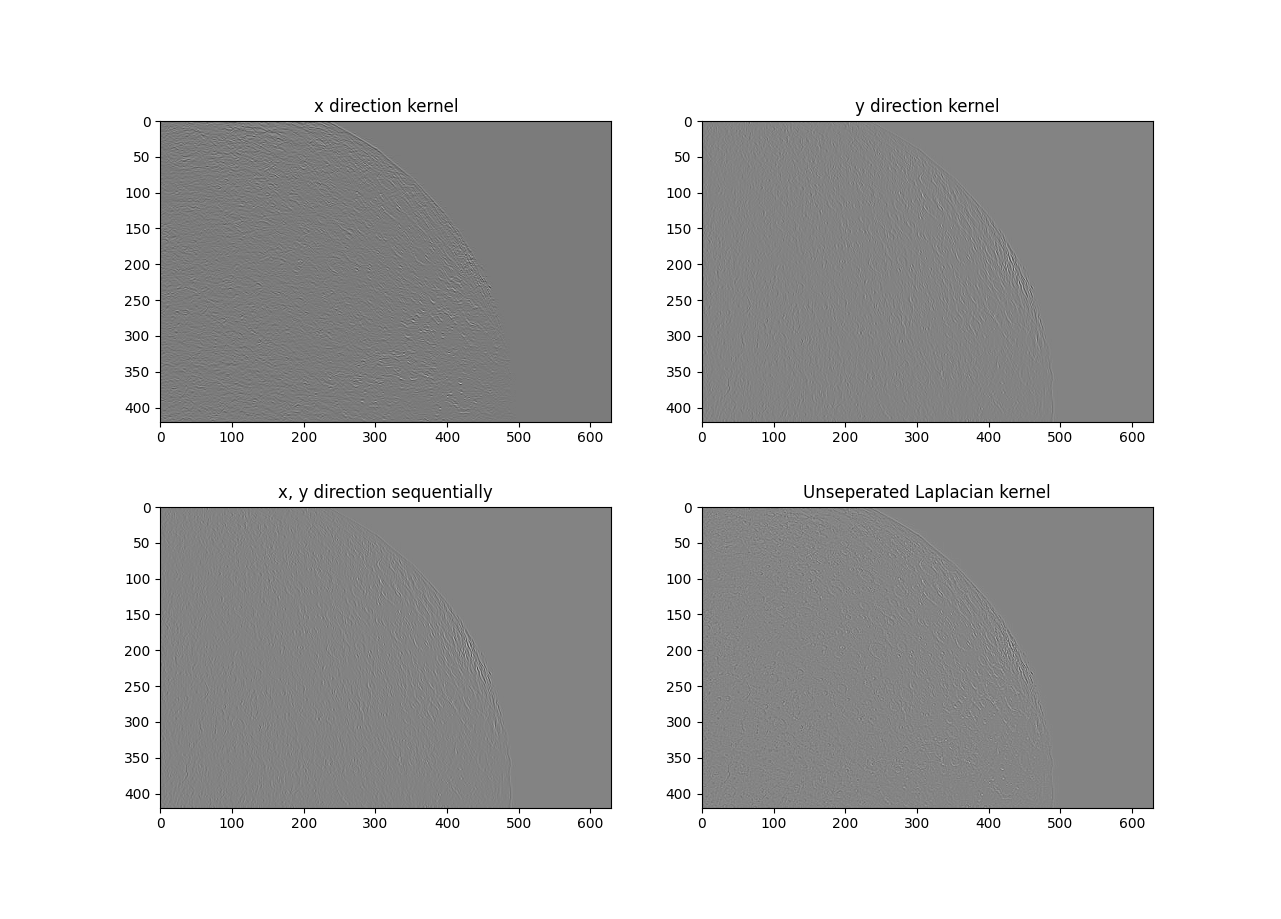
\includegraphics[width=1\textwidth]{../images/p2/p2a.png}
    \caption{Separated Laplacian kernels processed image}
\label{fig:p2a}
\end{figure}


(b) The Sharpened image with unseparated Laplacian kernel is shown in Figure \ref{fig:p2b}.\\
And all pixel intensity of the result images are normalized to uint8 values within $[0,255]$.\\

\begin{figure}[htbp]
    \centering
	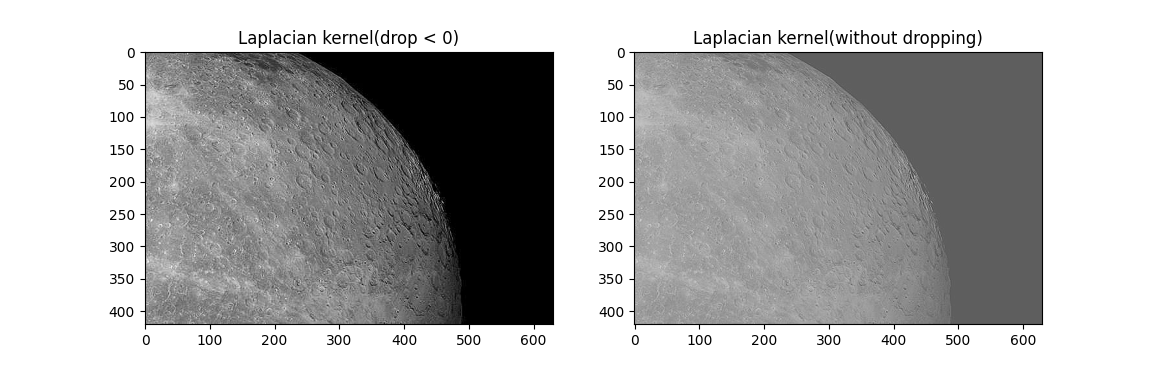
\includegraphics[width=\textwidth]{../images/p2/p2b.png}
    \caption{Unseparated Laplacian kernel processed image}
\label{fig:p2b}
\end{figure}

(c) The Sharpened image with unsharpen mask is shown in Figure \ref{fig:p2c}.\\
The left column is smoothed with the kernel 
$$\text{kernel\ 1}=\dfrac{1}{9}\begin{bmatrix}1 & 1 & 1\\1 & 1 & 1\\1 & 1 & 1\end{bmatrix}$$

And the right column is smoothed with the kernel
$$\text{kernel\ 2}=\dfrac{1}{16}\begin{bmatrix}1 & 2 & 1\\2 & 4 & 2\\1 & 2 & 1\end{bmatrix}$$

Suppose the origin image is $f(x,y)$.\\
The first row are the smoothed images processed by kernel1 and kernel2, mark as $\overline{f(x,y)}$.\\
The second row are the unsharped masks processed by kernel1 and kernel2. i.e. the difference between the
origin image and the smoothed image. i.e. $g_{mask}(x,y)=f(x,y)-\overline{f(x,y)}$.\\
The third and the forth rows are the sharpened images with different $k$. i.e. $g(x,y)=f(x,y)+k\cdot g_{mask}(x,y)$\\
The third row is the sharpened image with $k=1$, and the forth row is the sharpened image with $k=4.5$.\\

And all pixel intensity of the result images are normalized to uint8 values within $[0,255]$.\\
\begin{figure}[htbp]
    \centering
	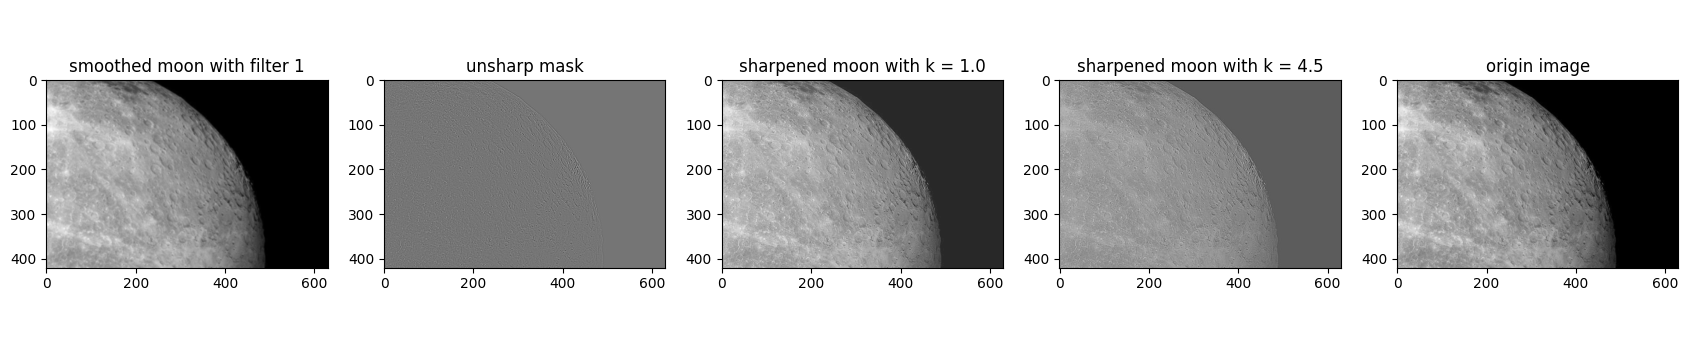
\includegraphics[width=\textwidth]{../images/p2/p2c_1_no_drop.png}
	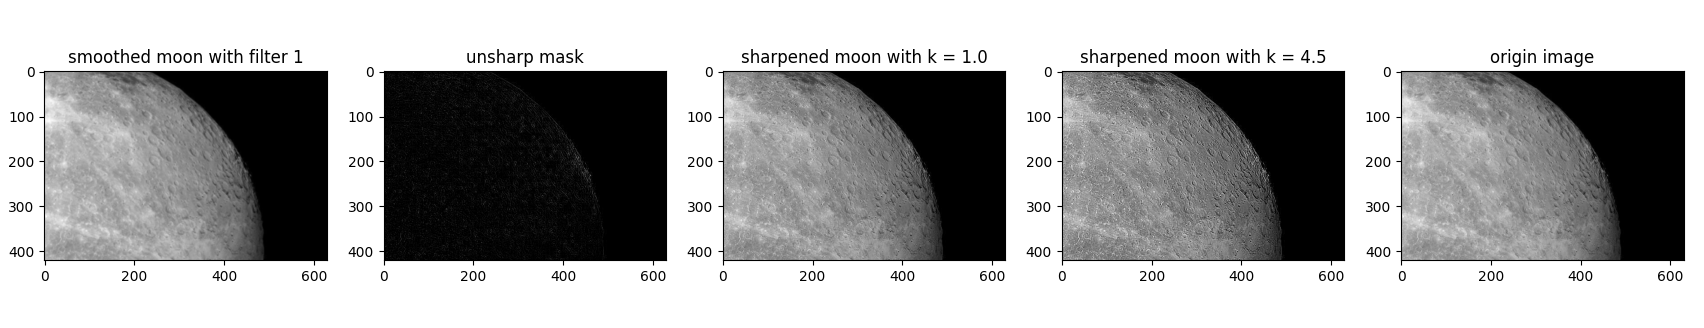
\includegraphics[width=\textwidth]{../images/p2/p2c_1_drop.png}
    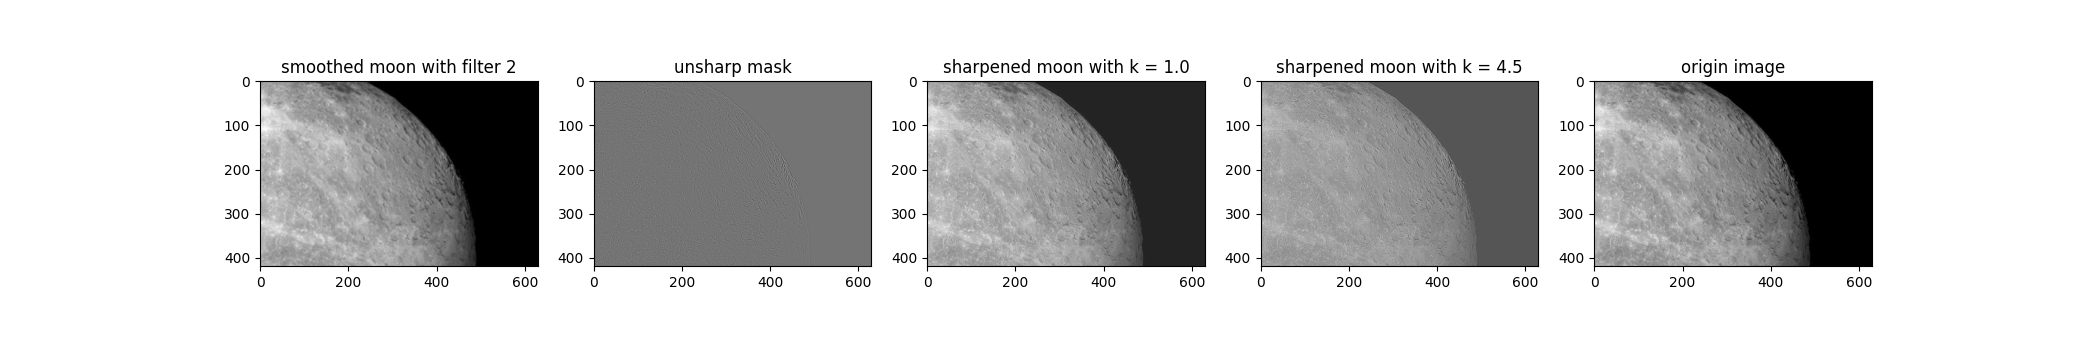
\includegraphics[width=\textwidth]{../images/p2/p2c_2_no_drop.png}
	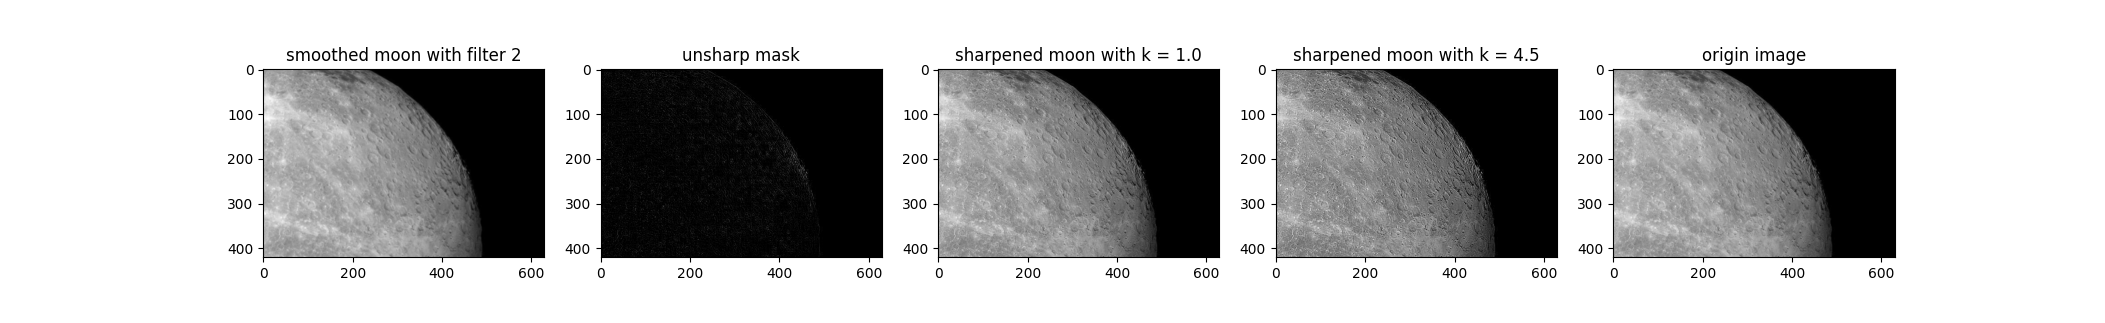
\includegraphics[width=\textwidth]{../images/p2/p2c_2_drop.png}
    \caption{unsharpen mask processed image}
\label{fig:p2c}
\end{figure}

\newpage